\subsection{Isomorphism in $\mathbb{R}$}
We have successfully constructed an isomorphism $\phi: \mathbb{Q_F} \rightarrow \mathbb{Q}$ that preserves all the important conditions (order, addition and multiplication), but our main goal is to extend this to all $\mathbb{R}$, starting from all $\mathbb{F}$.

So we expect a:
$$\Phi: \mathbb{F} \rightarrow \mathbb{R}$$

Such that:

\begin{enumerate}
\item Matches the former $\phi$ for all $\mathbb{Q_F}$ into $\mathbb{Q}$
\item Remains an isomorphism
\item Preserves the field's struture (order, addition and multiplication)
\end{enumerate}

The intuiton to create $\Phi$ was actually mentioned previously, on \cref{ex:s-in-q-not-bounded}. We talked about how a subset $S$ of an ordered field $\mathbb{Q}$ was bounded above by $\sqrt{2}$. The example talks more about how this $S$ won't have a supremum, but the key idea we will be using is how this particular $S$ was \textbf{bounded} by an irrational like $\sqrt{2}$. This is the relationship we need to apply to link irrational and rational numbers: \textbf{the first one bounds the second one}

With this idea, we can intuit that any \textbf{real number is actually defined by the numbers below it}. Take $\sqrt{2}$ for example:

\begin{enumerate}
\item $\sqrt{2}$ is greater than all the rationals $q$ where $q < \sqrt{2}$: 1, 1.4, 1.41, 1.414, \dots
\item $\sqrt{2}$ is less than all the rationals $q$ where $q > \sqrt{2}$: 2, 1.5, 1.42, 1.4145, \dots
\end{enumerate}

The fact is that $\sqrt{2}$ is the only number placed in the boundary between these to sequences.

More formally:
$$\sqrt{2} := \sup \{q \in \mathbb{Q}: q < \sqrt{2}\}$$
Relating an irrational number, with all the rationals below it.

\begin{definition}[$\Phi$ function]\label{def:Phi-function}
For any $\alpha \in \mathbb{R}$, define $\Phi: \mathbb{R} \rightarrow \mathbb{F}$ as
$$\Phi(\alpha) := \sup\{\phi(q): q \in \mathbb{Q}, q < \alpha \}$$
\end{definition}

This new function $\Phi$ using the former isomorphism $\phi$ defined in $\mathbb{Q}$ does the exact same thing that $\sqrt{2}$ did in our example: bounds $\mathbb{Q}$. Since our main focus is to somehow extend the properties of the original $\phi$, lets take the time to emphazise why this new $\Phi$ is not just an arbitrary function.

\begin{lemma}
For $r \in \mathbb{Q}$
\begin{align*}
\Phi(r)  = \phi(r)
\end{align*}
\end{lemma}

\begin{bookproof}
First, lets check the definition:
$$\Phi(\alpha) := \sup\{\phi(q): q \in \mathbb{Q}, q < \alpha \}$$

If $\alpha$ happens to be a rational number $r$, it means that the supremum of all the rational values before this particular $r$ are limited by $\phi(r)$, and this is the \textit{Least Upper Bound} of the set.

\begin{enumerate}
\item $\phi(r)$ bounds $\{\phi(q): q \in \mathbb{Q}, q < r \}$\\\\
Knowing that $\phi$ preserves order:
\begin{align*}
\forall q, q < r &\leftrightarrow \phi (q) < \phi (r)\\
&\leftrightarrow \phi(q) \leq \phi(r)
\end{align*}
$\Rightarrow \phi(r)$ bounds the set.
\end{enumerate}
\end{bookproof}

\begin{bookproof}
\begin{enumerate}
\setcounter{enumi}{1}
\item $\phi(r)$ is the L.U.B. of $\{\phi(q): q \in \mathbb{Q}, q < r \}$
\\\\
Lets visualize the approach

\begin{figure}[H]
\centering
\small
\begin{tikzcd}[column sep=scriptsize, row sep=small, scale=0.85]
	&&&&&&&&& {\textit{LUB}} \\
	{\mathbb{Q}} & {q_1} & {q_2} & \dots & q && {} & {q^\prime} & r & {} \\
	\\
	\\
	{\mathbb{Q}_F} & {\phi(q_1)} & {\phi(q_2)} & \dots & {\phi(q)} && M & {\phi(q^\prime)} & {\phi(r)} & {} \\
	&&&&& {} &&&& {}
	\arrow[shift right=4, from=2-1, to=2-10]
	\arrow["\phi"{description}, Rightarrow, from=2-1, to=5-1]
	\arrow[from=2-2, to=5-2]
	\arrow[from=2-3, to=5-3]
	\arrow[from=2-5, to=5-5]
	\arrow["{{\epsilon_M/2}}"{description}, shift left=5, between={0.3}{0.7}, no head, from=2-7, to=2-10]
	\arrow[from=2-8, to=5-8]
	\arrow[shift left=2, curve={height=18pt}, between={0}{0.9}, from=2-9, to=1-10]
	\arrow[from=2-9, to=5-9]
	\arrow[shift left=4, from=5-1, to=5-10]
	\arrow["{{\epsilon_M}}"{description}, shift left=2, between={0.2}{0.8}, no head, from=6-6, to=6-10]
\end{tikzcd}
\end{figure}


Assume $M$ is an arbitrary upper bound, trying to make $\phi(r)$ not the \textit{L.U.B.}
\begin{align*}
\rightarrow M < \phi(r)
\rightarrow \phi(r) - M > 0
\end{align*}
Lets call $\epsilon_M$ to the distance between this assumed $M$ and $\phi(r)$.

Now, lets not forget that by density in $\mathbb{Q}$ we are able to locate an arbitrary rational number between two other arbitrary rationals, or even better for our use case: we can position an arbitrary rational $q^\prime$ as close as we want to any other arbitrary rational.

Developing that idea:
\begin{align*}
\forall \ r \in \mathbb{Q}, \exists \ q^\prime \in \mathbb{Q} : q^\prime - \epsilon \leq r, \epsilon \in \mathbb{Q}
\end{align*}

Now, $M \in \mathbb{Q_F}$, but the density propery we are using for $q^\prime$ is in $\mathbb{Q}$. Luckily, we already proved that $\phi$ is ordered:


\begin{align*}
\forall \ r \in \mathbb{Q}&, \exists \ q^\prime \in \mathbb{Q} / \forall \epsilon > 0: q^\prime - \epsilon \leq r \\
&\rightarrow \phi(q^\prime) - \phi(\epsilon) \leq \phi(r)
\end{align*}

Now that we are entirely in $\mathbb{Q_F}$ we will conveniently take this distance $\phi(\epsilon)$ as $\epsilon_M / 2$, just to note that this will be smaller than the distance between $M$ and $r$. No matter how close we assume $M$ is to $\phi(r)$, by density in $\mathbb{Q}$ we can make sure that we can take half that distance (or a quarter, or a tenth, doesn't matter) to locate another image closer to $\phi(r)$.

\begin{align*}
\rightarrow M < \phi(q^\prime) < \phi(r)
\rightarrow M \neq \text{ Upper bound}
\end{align*}
$$\Rightarrow \Phi(r) := \sup\{\phi(q): q \in \mathbb{Q}, q < r \} = \phi(r), \ \forall r \in \mathbb{Q}$$
\end{enumerate}
\end{bookproof}	

Taking the time to proof this mapping for rationals wasn't a waste of time after all, since it confirms that our intuition about the definition of $\Phi$ isn't arbitrary, but respects the structure we already built.


\subsubsection{Completeness of $\Phi$}

So far, our definition for $\Phi$:

$$\Phi(\alpha) := \sup\{\phi(q): q \in \mathbb{Q}, q < \alpha \}$$

Uses an internal set $S(\alpha) = \{\phi(q): q \in \mathbb{Q}, q < \alpha \}$ that we can use to simplify our readability a bit:

$$\Phi(\alpha) := \sup(S(\alpha))$$

Now, to make $\Phi$ to make sense we need to make sure that $S$ makes sense, and if we want to obtain the supremum of a poorly-define set, the whole definition crumbles.

Next, we will review how $S(\alpha)$ is well defined to avoid any issues further down.

\begin{lemma}
Set $S$:
$$\Phi(\alpha) := \sup\{S(\alpha)\} = \sup\{\phi(q): q \in \mathbb{Q}, q < \alpha \}$$ is well defined in $\mathbb{R}$
\end{lemma}

\begin{bookproof}
To proof this, what matters the most is that $S$ is well-defined in $\mathbb{F}$. That automatically guarantees that $\Phi$ makes sense in $\mathbb{R}$.
\begin{enumerate}
\item $S(\alpha)$ is not empty:

Using \cref{th:archimedean} (Archimedean theorem):
\begin{align*}
&\forall \alpha \in \mathbb{Q}, \exists \ n \in \mathbb{N}: n > \alpha \\
&\rightarrow n > |\alpha| \\
&\rightarrow -n < \alpha, -n \in \mathbb{Q}
\end{align*}
Identifying $q = -n$ in $S$, we have a rational that is bounded by $\alpha$, meaning that $\phi(-n) \in S(\alpha)$
\\
\item $S(\alpha)$ is bounded above:

Again, using \cref{th:archimedean}:
\begin{align*}
&\forall \alpha \in \mathbb{Q}, \exists \ n \in \mathbb{N}: n > \alpha \\
\end{align*}
Then, for any rational $q < \alpha$
\begin{align*}
& n > \alpha > q \\
& \rightarrow q < n \\
& \rightarrow \phi(q) < \phi(n) = n_\mathbb{F}\\
\end{align*}
So $n_\mathbb{F}$ is an upper bound of $S$, for any $q < \alpha$
\end{enumerate}
$\rightarrow S(\alpha)$ is well-defined in $\mathbb{F}$ \\\\
$\rightarrow \Phi(\alpha) := \sup\{S(\alpha)\}$ is well-defined in $\mathbb{R}$
\end{bookproof}

Now, while studying this a question came to me: if we already know that $\phi: \mathbb{Q} \rightarrow \mathbb{Q_F}$ exists, why do we need to prove $S(\alpha)$ is non-empty? Can't we just pick any rational and map it?


The issue is that the set $S(\alpha)$ is not just any images of rationals, it's specifically:
$S(\alpha) = \{\phi(q) : q \in \mathbb{Q} \text{ AND } q < \alpha\}$. The constraint $q < \alpha$ obligues us to prove that \textit{there exists at least one rational $q$ with $q < \alpha$}.

\begin{lemma}[Order-Preservation]\label{le:order-Phi}
For $\alpha, \beta \in \mathbb{R}$

$$\alpha < \beta \rightarrow \Phi(\alpha) < \Phi(\beta)$$
\end{lemma}

\begin{bookproof}
Lets start with two evaluations of set $S$:
\begin{itemize}
\item $S(\alpha) := \{\phi(q): q \in \mathbb{Q}, q < \alpha \}$
\item $S(\beta) := \{\phi(q): q \in \mathbb{Q}, q < \beta \}$
\end{itemize}

If $\alpha < \beta$, then for any $\phi(q^\prime) \in S(\alpha)$:
\begin{align*}
\phi(q) \in S(\alpha) &\leftrightarrow \phi(q^\prime) \in \{\phi(q): q \in \mathbb{Q}, q < \alpha \} \\
&\leftrightarrow \phi(q^\prime) \in \{\phi(q): q \in \mathbb{Q}, q < \alpha < \beta \} \\
&\leftrightarrow \phi(q^\prime) \in \{\phi(q): q \in \mathbb{Q}, q < \beta \} \\
&\leftrightarrow \phi(q^\prime) \in S(\beta)
\end{align*}

Then, going back to the statement:

\begin{align*}
\alpha < \beta &\Rightarrow S(\alpha) \subseteq S(\beta) \\
&\Rightarrow \sup(S(\alpha)) \leq \sup(S(\beta)) \\
&\Rightarrow \Phi(\alpha) \leq \Phi(\beta)
\end{align*}

Now, to prove that the images of $\alpha$ and $\beta$ in $\Phi$ are strictly less than and not equal, we use the density of $\mathbb{Q}$ in $\mathbb{R}$ to locate arbitrary rationals $r_\alpha, r_\beta$.
\begin{align*}
\forall \alpha, \beta \in \mathbb{R}, \exists \ r_\alpha, r_\beta \in \mathbb{Q}: \\
\alpha < \beta \rightarrow  \alpha < r_\alpha < r_\beta < \beta \\
\end{align*}

Since $r_\beta < \beta \rightarrow \phi(r_\beta) \in S(\beta)$ by the definition of $S$. Now, knowing that for any element of $S(\beta)$ it will be less or equal to its supremum, we have:
\begin{align*}
\phi(r_\beta) \leq \sup(S(\beta)) \\
\phi(r_\beta) \leq \Phi(\beta)
\end{align*}

Now in the middle, by order preservation:
\begin{align*}
r_\alpha < r_\beta \leftrightarrow \phi(r_\alpha) < \phi(r_\beta)
\end{align*}

And finally, since $\alpha < r_\alpha \rightarrow S(\alpha) \subseteq S(r_\alpha)$. Then:

\begin{align*}
&S(\alpha) \subseteq S(r_\alpha) \\
&\rightarrow \Phi(\alpha) \leq \Phi(r_\alpha) \\
&\rightarrow \Phi(\alpha) \leq \phi(r_\alpha) \text{ (Since $r_\alpha \in \mathbb{Q}$)} \\
\end{align*}

Joining all results:
\begin{align*}
\Phi(\alpha) &\leq \phi(r_\alpha) < \phi(r_\beta) \leq \Phi(\beta) \\
&\Rightarrow \Phi(\alpha) < \Phi(\beta) \\
\end{align*}

Finally, $\alpha < \beta \Rightarrow \Phi(\alpha) < \Phi(\beta)$.
\end{bookproof}

Now comes the final sprint to proof that $\Phi$ maps $\mathbb{F}$ and $\mathbb{R}$ perfectly. Just as we did with $\phi$, we need to prove isomorphism by proving bijection and homomorphism. From this last part, the only tricky step is for surjectiveness, since it uses a method that we haven't seeing before. We are almost there!

\begin{lemma}[Injectivity in $\Phi$]
Given $\Phi: \mathbb{R} \rightarrow \mathbb{F}$
, for $\alpha, \beta \in \mathbb{R}:$
$$\alpha \neq \beta \rightarrow \Phi(\alpha) \neq \Phi(\beta)$$
\end{lemma}

\begin{bookproof}
From proven order preservation in \cref{le:order-Phi}, if $\alpha \neq \beta$
\begin{enumerate}
\item $\alpha < \beta \rightarrow \Phi(\alpha) < \Phi(\beta) \rightarrow \Phi(\alpha) \neq \Phi(\beta)$
\item $\alpha > \beta \rightarrow \Phi(\alpha) > \Phi(\beta) \rightarrow \Phi(\alpha) \neq \Phi(\beta)$ 
\end{enumerate}
\end{bookproof}

\begin{lemma}[Surjectivity in $\Phi$]
Given $\Phi: \mathbb{R} \rightarrow \mathbb{F}$:
$$\forall \  a \in \mathbb{F},\exists \ \alpha \in \mathbb{R}: \Phi(\alpha) = a$$
\end{lemma}

\begin{bookproof}
Lets support the following ideas on the next diagram:
\begin{center}
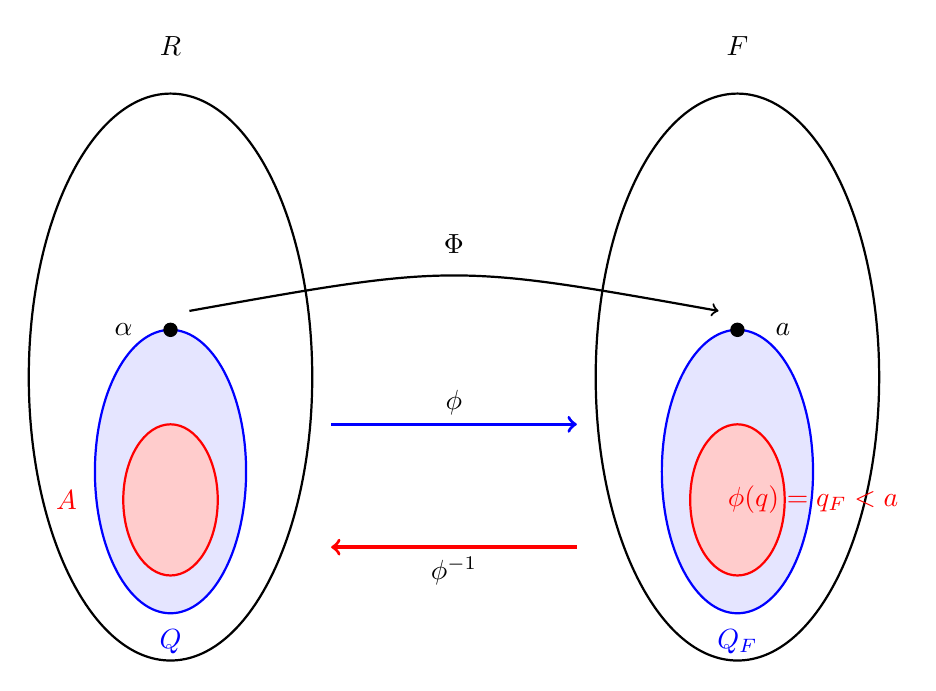
\begin{tikzpicture}[scale=1.2]
    % Left set (R)
    \draw[thick] (-2,0) ellipse (1.5cm and 3cm);
    \node at (-2, 3.5) {$\mathbb{R}$};
    
    % Right set (F)
    \draw[thick] (4,0) ellipse (1.5cm and 3cm);
    \node at (4, 3.5) {$\mathbb{F}$};
    
    % Rationals in R (highlighted region)
    \draw[thick, blue, fill=blue!10] (-2,-1) ellipse (0.8cm and 1.5cm);
    \node[blue] at (-2, -2.8) {$\mathbb{Q}$};
    
    % Rationals in F (highlighted region)
    \draw[thick, blue, fill=blue!10] (4,-1) ellipse (0.8cm and 1.5cm);
    \node[blue] at (4, -2.8) {$\mathbb{Q}_F$};
    
    % Set A (the preimage)
    \draw[thick, red, fill=red!20] (-2,-1.3) ellipse (0.5cm and 0.8cm);
    \node[red] at (-3.1, -1.3) {$A$};
    
    % Elements below a in Q_F
    \draw[thick, red, fill=red!20] (4,-1.3) ellipse (0.5cm and 0.8cm);
    \node[red] at (4.8, -1.3) {$\phi(q) = q_\mathbb{F} < a$};
    
    % Alpha (supremum of A)
    \filldraw[black] (-2, 0.5) circle (2pt);
    \node[left] at (-2.3, 0.5) {$\alpha$};
    
    % a in F
    \filldraw[black] (4, 0.5) circle (2pt);
    \node[right] at (4.3, 0.5) {$a$};
    
    % Phi arrow (forward)
    \draw[->, very thick, blue] (-0.3, -0.5) -- (2.3, -0.5);
    \node[above] at (1, -0.5) {$\phi$};
    
    % Phi inverse arrow (backward)
    \draw[->, very thick, red] (2.3, -1.8) -- (-0.3, -1.8);
    \node[below] at (1, -1.8) {$\phi^{-1}$};
    
    % Phi arrow from alpha to a
    \draw[->, thick, black] (-1.8, 0.7) .. controls (1, 1.2) .. (3.8, 0.7);
    \node[above] at (1, 1.2) {$\Phi$};
\end{tikzpicture}
\end{center}


Picking an arbitrary $a \in \mathbb{Q_F}$, we define the subset bounded above by this $a$:
$$\{\phi(q) = q_\mathbb{F} \in \mathbb{Q_F}, q_\mathbb{F} < a\}$$

Now, since we already know that $\phi$ is a isomorphism (and hence, is injective), we know that its inverse $\phi ^{-1}$ exists. Applying it to the defined set we create $A$:

\begin{align*}
A &= \phi ^{-1}(\{q_\mathbb{F} \in \mathbb{Q_F}, q_\mathbb{F} < a\}) \\
&= \phi ^{-1}(\{\phi(q), q \in \mathbb{Q}, \phi(q) < a\}) \\
&= \{q \in \mathbb{Q}, \phi(q) < a\})
\end{align*}

Now lets consider $\alpha = \sup(A)$, lets first prove that $\alpha$ exists:

\begin{enumerate}
\item $A$ is non-empty:

Let an arbitrary $q \in \mathbb{Q}$, then $\phi(q) = q_\mathbb{F} \in \mathbb{Q_F}$. This means that $\phi(q) < a$, and by definition of $A$, $q \in A$.

\item $A$ is bounded above:

Using the archimedean property in $\mathbb{F}: \exists n_\mathbb{F} \in \mathbb{N_\mathbb{F}}: n_\mathbb{F} > a$. But from the definition of $A, \exists q \in \mathbb{Q}: \phi(q) < a$. Then $\phi(a) < a < n_\mathbb{F}$. Since $\phi$ is order-preserving, we evaluate its inverse in the interval and get $\phi^{-1}(\phi(a)) < \phi^{-1}(n_\mathbb{F})$. Then, $a < n$ shows that $n$ is an upper bound for $A$.
\end{enumerate}

$\Rightarrow \alpha = \sup(A)$ exists
\end{bookproof}

\begin{bookproof}
Now, want we want to achieve is that given this arbitrary $a$, we reach the preimage $\alpha$ by expanding se $A$ enough to declare that $\alpha$ is its supremum. That way, we match the definition of $\Phi$ and that would be it.
\\\\
Claim: $$\{q \in \mathbb{Q}: q < \alpha\} = A$$

\begin{itemize}
\item $\subseteq$:

Let $q \in \mathbb{Q}: q < \alpha$. If we fix an arbitrary $q^\prime \in A$ and using the fact that $\alpha = \sup(A)$, then there is an $\epsilon$ small enough (the minimal in fact) that $q^\prime + \epsilon > \alpha$. Now, ordering:

\begin{align*}
&q < q^\prime < \alpha &\text{ (choosing the smallest $\epsilon$)} \\
&\rightarrow q < q^\prime \\
&\rightarrow \phi(q) < \phi(q^\prime) &\text{ (due $\phi$ preserving order)}
\end{align*}

Since $\phi(q^\prime) \in \mathbb{Q_F}$, $\phi(q^\prime) < a$ (as the diagram implies from our initial assumptions)

$$\rightarrow \phi(q) < \phi(q^\prime) < a$$
$$\rightarrow q \in A$$

\item $\supseteq$:

Let $q \in A$. By definition, $\phi(q) < a$ and, since $\alpha = \sup(A), q < \alpha$.

$$\rightarrow q \in \{q \in \mathbb{Q}: q < \alpha\}$$
\end{itemize}

$$\Rightarrow \{q \in \mathbb{Q}: q < \alpha\} = A$$

So far we proved that:
\begin{enumerate}
\item $\sup(A) = \alpha$ exists
\item $A = \{q \in \mathbb{Q}: q < \alpha\}$
\end{enumerate}

Lets combine the two:

$$
\sup(A) = \sup\{q \in \mathbb{Q}: q < \alpha\}
$$

And from the definition:
\begin{align*}
\Phi(\alpha) &= \sup\{\phi(q), q \in \mathbb{Q}, q < \alpha\} \\
&= \sup\{\phi(q), q \in A\} \\
\end{align*}

But from the original definition of $A = \phi ^{-1}(\{q_\mathbb{F} \in \mathbb{Q_F}, q_\mathbb{F} < a\})$, and replacing:

\end{bookproof}
